% Native TikZ figure for the n=7 local move.  The surrounding manuscript
% supplies tikz and xcolor; this file is intentionally not standalone.
\begin{figure}[htbp]
  \centering
  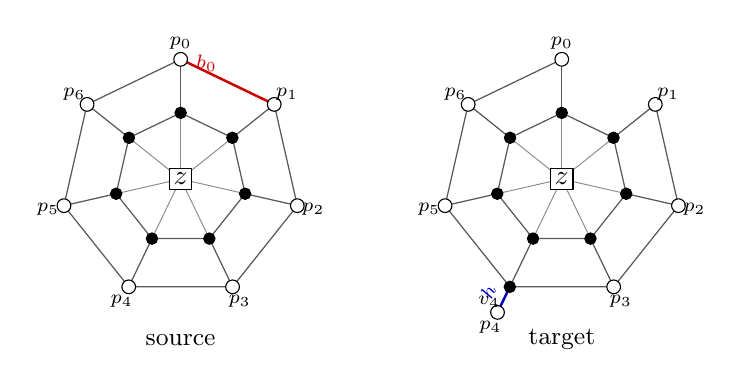
\begin{tikzpicture}[
    scale=.8,
    line join=round,
    edge/.style={draw=black!65, line width=.45pt},
    centeredge/.style={draw=black!45, line width=.35pt},
    internal/.style={circle, draw=black, fill=black, inner sep=1.45pt},
    port/.style={circle, draw=black, fill=white, inner sep=1.75pt, minimum size=4.5pt},
    centerport/.style={rectangle, draw=black, fill=white, inner sep=1.5pt, minimum size=6pt},
    labelstyle/.style={font=\scriptsize},
    bzero/.style={draw=red!80!black, line width=.9pt},
    hspike/.style={draw=blue!75!black, line width=.9pt}
  ]

    % ------------------------------------------------------------------
    % Source: seven observed outer ports, seven internal inner vertices,
    % and the observed centre z.
    % ------------------------------------------------------------------
    \begin{scope}
      \coordinate (sU0) at (90:1.05);
      \coordinate (sU1) at ({90-360/7}:1.05);
      \coordinate (sU2) at ({90-720/7}:1.05);
      \coordinate (sU3) at ({90-1080/7}:1.05);
      \coordinate (sU4) at ({90-1440/7}:1.05);
      \coordinate (sU5) at ({90-1800/7}:1.05);
      \coordinate (sU6) at ({90-2160/7}:1.05);
      \coordinate (sP0) at (90:1.9);
      \coordinate (sP1) at ({90-360/7}:1.9);
      \coordinate (sP2) at ({90-720/7}:1.9);
      \coordinate (sP3) at ({90-1080/7}:1.9);
      \coordinate (sP4) at ({90-1440/7}:1.9);
      \coordinate (sP5) at ({90-1800/7}:1.9);
      \coordinate (sP6) at ({90-2160/7}:1.9);
      \coordinate (sZ) at (0,0);

      % Centre spokes, inner cycle, radial edges, and outer cycle.
      \foreach \i in {0,...,6} {
        \draw[centeredge] (sZ) -- (sU\i);
      }
      \draw[edge] (sU0)--(sU1)--(sU2)--(sU3)--(sU4)--(sU5)--(sU6)--cycle;
      \draw[edge] (sU0)--(sP0);
      \draw[edge] (sU1)--(sP1);
      \draw[edge] (sU2)--(sP2);
      \draw[edge] (sU3)--(sP3);
      \draw[edge] (sU4)--(sP4);
      \draw[edge] (sU5)--(sP5);
      \draw[edge] (sU6)--(sP6);
      \draw[edge] (sP0)--(sP1)--(sP2)--(sP3)--(sP4)--(sP5)--(sP6)--cycle;
      \draw[bzero] (sP0) -- node[midway, above left, labelstyle, text=red!80!black] {$b_0$} (sP1);

      \node[internal] at (sU0) {};
      \node[internal] at (sU1) {};
      \node[internal] at (sU2) {};
      \node[internal] at (sU3) {};
      \node[internal] at (sU4) {};
      \node[internal] at (sU5) {};
      \node[internal] at (sU6) {};
      \node[port] at (sP0) {};
      \node[port] at (sP1) {};
      \node[port] at (sP2) {};
      \node[port] at (sP3) {};
      \node[port] at (sP4) {};
      \node[port] at (sP5) {};
      \node[port] at (sP6) {};
      \node[centerport] at (sZ) {$z$};
      \node[labelstyle] at (90:2.16) {$p_0$};
      \node[labelstyle] at ({90-360/7}:2.16) {$p_1$};
      \node[labelstyle] at ({90-720/7}:2.16) {$p_2$};
      \node[labelstyle] at ({90-1080/7}:2.16) {$p_3$};
      \node[labelstyle] at ({90-1440/7}:2.16) {$p_4$};
      \node[labelstyle] at ({90-1800/7}:2.16) {$p_5$};
      \node[labelstyle] at ({90-2160/7}:2.16) {$p_6$};
      \node[font=\small] at (0,-2.55) {source};
    \end{scope}

    % ------------------------------------------------------------------
    % Target: b_0 is absent.  The old outer p_4 is the internal vertex v_4;
    % the new observed p_4 is farther out and is attached by the blue spike.
    % ------------------------------------------------------------------
    \begin{scope}[xshift=6.05cm]
      \coordinate (tU0) at (90:1.05);
      \coordinate (tU1) at ({90-360/7}:1.05);
      \coordinate (tU2) at ({90-720/7}:1.05);
      \coordinate (tU3) at ({90-1080/7}:1.05);
      \coordinate (tU4) at ({90-1440/7}:1.05);
      \coordinate (tU5) at ({90-1800/7}:1.05);
      \coordinate (tU6) at ({90-2160/7}:1.05);
      \coordinate (tP0) at (90:1.9);
      \coordinate (tP1) at ({90-360/7}:1.9);
      \coordinate (tP2) at ({90-720/7}:1.9);
      \coordinate (tP3) at ({90-1080/7}:1.9);
      \coordinate (v4) at ({90-1440/7}:1.9);
      \coordinate (tP4) at ({90-1440/7}:2.35);
      \coordinate (tP5) at ({90-1800/7}:1.9);
      \coordinate (tP6) at ({90-2160/7}:1.9);
      \coordinate (tZ) at (0,0);

      \foreach \i in {0,...,6} {
        \draw[centeredge] (tZ) -- (tU\i);
      }
      \draw[edge] (tU0)--(tU1)--(tU2)--(tU3)--(tU4)--(tU5)--(tU6)--cycle;
      \draw[edge] (tU0)--(tP0);
      \draw[edge] (tU1)--(tP1);
      \draw[edge] (tU2)--(tP2);
      \draw[edge] (tU3)--(tP3);
      \draw[edge] (tU4)--(v4);
      \draw[edge] (tU5)--(tP5);
      \draw[edge] (tU6)--(tP6);

      % The outer cycle with b_0 removed, and the two old p_4 incidences
      % redirected to the internal v_4.
      \draw[edge] (tP1)--(tP2)--(tP3)--(v4)--(tP5)--(tP6)--(tP0);
      \draw[hspike] (v4) -- node[midway, sloped, above, labelstyle, text=blue!75!black] {$h$} (tP4);

      \node[port] at (tP0) {};
      \node[port] at (tP1) {};
      \node[port] at (tP2) {};
      \node[port] at (tP3) {};
      \node[port] at (tP4) {};
      \node[port] at (tP5) {};
      \node[port] at (tP6) {};
      \node[internal] at (tU0) {};
      \node[internal] at (tU1) {};
      \node[internal] at (tU2) {};
      \node[internal] at (tU3) {};
      \node[internal] at (tU4) {};
      \node[internal] at (tU5) {};
      \node[internal] at (tU6) {};
      \node[internal] at (v4) {};
      \node[labelstyle, below left] at (v4) {$v_4$};
      \node[centerport] at (tZ) {$z$};
      \node[labelstyle] at (90:2.16) {$p_0$};
      \node[labelstyle] at ({90-360/7}:2.16) {$p_1$};
      \node[labelstyle] at ({90-720/7}:2.16) {$p_2$};
      \node[labelstyle] at ({90-1080/7}:2.16) {$p_3$};
      \node[labelstyle] at ({90-1440/7}:2.61) {$p_4$};
      \node[labelstyle] at ({90-1800/7}:2.16) {$p_5$};
      \node[labelstyle] at ({90-2160/7}:2.16) {$p_6$};
      \node[font=\small] at (0,-2.55) {target};
    \end{scope}
  \end{tikzpicture}
  \caption{The full $n=7$ source and target before common boundary stripping.
    The move deletes the outer edge $b_0=p_0p_1$ and
    replaces the opposite outer vertex by an internal vertex $v_4$ with a
    new observed port $p_4$ attached by the spike $h$.  White vertices,
    including the boxed centre port $z$, are observed;
    black dots are internal vertices.}
  \label{fig:seven-move}
\end{figure}
